\section{Introduction}\label{sec:1}

The competition scores an agent bundle on hidden GitHub-issue tasks, with Gemma 4 served by vLLM \cite{r11}. Third-party analyses put the noise of one hosted score near 1.5 of 58 tasks \cite{r3,r4}. Local evaluation must therefore carry development; on a Kaggle kernel with four L4 GPUs our stack finished 35.2 agent runs per hour, serially.

\textbf{Safety.} An agent run executes model-written shell commands and installs model-edited packages; our first local setup ran them with no sandbox.

\textbf{Fidelity.} We call a \emph{rendering trap} a configuration detail that silently changes the token sequence the model receives while runs still finish and score. The \emph{scorer path} is the scorer's configuration reproduced locally. In our first setup the served model name contained ``gemma4'', so the agent framework (google-adk 1.36.1) sent tool results with role \texttt{tool\_responses} instead of \texttt{tool} \cite{r5}. Prompts rebuilt from its traces matched the server's token counts on 106 of 114 calls only when rendered with \texttt{tool\_responses} (0 of 114 with \texttt{tool}). Solve counts hid it: that setup solved 3 and 5 of 24 tasks against 4 and 4 on Kaggle (Fisher p 0.74 and 0.75).

These traps are public: the role rule \cite{r5}, thought handling in history \cite{r6,r7,r8}, a newline after thinking text \cite{r9}, and the scorer's compaction settings \cite{r10}. We discovered none of them; we contribute checks that detect them (\S\ref{sec:4}) and a measurement of three of them plus a template swap (\S\ref{sec:6}).

\section{Scope, threat model and rules}\label{sec:2}

% Figure: where the three modules sit. Every label restates Sections 3-5; no number here is new.
\begin{figure}[!tb]
\centering
\footnotesize
\begin{tikzpicture}[
  box/.style={draw, rounded corners=2pt, align=center, inner sep=4pt, text width=#1, minimum height=0.95cm},
  con/.style={box=#1, fill=blue!8},
  cfm/.style={box=#1, fill=green!12},
  cmp/.style={box=#1, fill=orange!16},
  plain/.style={box=#1, fill=white},
  arr/.style={-{Stealth[length=1.8mm]}, thick},
  darr/.style={{Stealth[length=1.8mm]}-{Stealth[length=1.8mm]}, thick},
  lab/.style={font=\scriptsize, align=center, inner sep=1.5pt, text=black!75}]
% row 1: what starts a job
\node[plain=2.5cm] (jobs)   at (1.2,0)    {job list: task $\times$ arm $\times$ repeat};
\node[con=3.9cm]   (runner) at (5.6,0)    {\textbf{runner} (trusted): starts agent runs only if eight recorded hashes match};
% row 2: the job
\node[lab, anchor=south] (ctrlab) at (5.05,-1.93) {one fresh container per job};
\node[plain=2.25cm] (agent) at (3.6,-2.55) {agent: framework and bundle};
\node[plain=2.25cm] (repo)  at (6.5,-2.55) {task repository and its tests};
\node[lab, anchor=north, text width=5.5cm] (restr) at (5.05,-3.2)
  {no network, no capabilities, seccomp filter, read-only root, unprivileged user; CPU, memory, process and file caps};
\begin{scope}[on background layer]
\node[draw, dashed, rounded corners=3pt, fill=blue!8, inner xsep=7pt, inner ysep=4pt, fit=(ctrlab)(agent)(repo)(restr)] (ctr) {};
\end{scope}
\node[con=2.45cm] (fwd) at (11.55,-2.55) {\textbf{forwarder}: chat requests only, allow-listed fields, approved template};
\node[plain=1.75cm] (srv) at (14.75,-2.55) {model server on one GPU};
% row 3: what reads the outputs
\node[cmp=5.5cm] (cmpn) at (5.05,-6.0)  {\textbf{compare}: candidate against baseline on the same tasks and repeats; repository clusters; frozen pass rule};
\node[cfm=5.2cm] (cfmn) at (13.15,-6.0) {\textbf{conform}: eight checks of requests and rendered prompts against the scorer path, down to token ids};
% arrows
\draw[arr] (jobs) -- (runner);
\draw[arr] (runner.south) -- node[lab, right, xshift=1pt] {starts, grades} (runner.south |- ctr.north);
\draw[darr] (repo.east) -- (fwd.west);
\path (ctr.east |- repo.east) -- node[lab, above] {per-job} node[lab, below] {Unix socket} (fwd.west);
\draw[arr] (ctr.south) -- node[lab, right, xshift=1pt] {verdict rows} (ctr.south |- cmpn.north);
\draw[arr] (fwd.south) -- node[lab, left, xshift=-1pt] {requests} (fwd.south |- cfmn.north);
\draw[arr] (srv.south) -- node[lab, right, xshift=1pt, text width=1.3cm] {rendered prompts} (srv.south |- cfmn.north);
% module tag
\node[lab, anchor=south west, text=blue!50!black] at ([yshift=1pt]runner.north west) {\textbf{contain}};
\end{tikzpicture}
\caption{The kit: where each module sits.}
\label{fig:overview}
\end{figure}


\textbf{Stack.} Gemma 4 E4B, 4-bit quantization-aware checkpoint (Kaggle model version 2); vLLM 0.19.1; google-adk 1.36.1; the competition's harness packages. Tasks come from Berth \cite{r12}: 579 of its 653 tasks load in the harness and pass our validation (the reference patch passes, an empty patch fails). Experiments ran on a shared single-GPU workstation (RTX 5090, 32 GB).

\textbf{Threat model.} The adversary is the code the agent writes. It may try to read host files or other jobs, reach the network, exhaust host resources, forge its verdict, or outlive its job. Kernel exploits are out of scope.

\textbf{Who did the work.} AI agents wrote the kit's code, attacks and analyses (builders). Separate AI agents (verifiers) re-implemented or re-ran the work adversarially. A lead AI session froze the protocols; a human owner approved isolation, machine time and release. ``Verified'' below means this process, not human review.

\section{Contain: a runner and the attacks it failed}\label{sec:3}

In the final design each job gets one fresh container: no network, no capabilities, a seccomp filter, a read-only root, an unprivileged user, 2 CPUs, 10 GiB of memory, 4,096 processes, and temporary filesystems capped in bytes and inodes. The only request channel is a per-job Unix socket to a forwarder, which passes only chat-completion requests with allow-listed fields, text-only content and an approved template hash, under rate and size caps. Agent runs start only if eight recorded hashes (image, code, flags, model files) still match.

A \emph{canary} is a scripted attack with a machine-checked outcome.

\begin{table}[!tb]
\centering
\caption{Runner versions.}\label{tab:1}
\footnotesize
\begin{tabular}{@{}
  >{\raggedright\arraybackslash}p{(\linewidth - 4\tabcolsep) * \real{0.2000}}
  >{\raggedright\arraybackslash}p{(\linewidth - 4\tabcolsep) * \real{0.1900}}
  >{\raggedright\arraybackslash}p{(\linewidth - 4\tabcolsep) * \real{0.6100}}@{}}
\toprule
\begin{minipage}[b]{\linewidth}\raggedright
Runner version
\end{minipage} & \begin{minipage}[b]{\linewidth}\raggedright
Canaries passed
\end{minipage} & \begin{minipage}[b]{\linewidth}\raggedright
Security findings of independent verifiers
\end{minipage} \\
\midrule
1. Container per command & 52/52 & 4 high: host-side install ran the agent's \texttt{setup.py} (builder-found); symlink leaked a host file; 10 GiB of host disk reserved in 0.005 s; host copied a sparse file in full \\
2. Hardened, per command & 60/60 (57/60 before canary fixes) & 4 high, 1 untested: host overwrote a file through a planted link; cleanup followed links; 6 GiB reserved in 0.012 s; 200,000 files in 2.4 s \\
3. Container per job & 98/98 & 1 high: the model server could fetch URLs named in requests; 2 medium \\
4--6. Request filter added, tightened & 134/134, 159/159, 191/191 & medium at most \\
7. Final & 200/200 & no high or medium \\
\bottomrule
\end{tabular}
\end{table}

\begin{figure}[!tb]
\centering
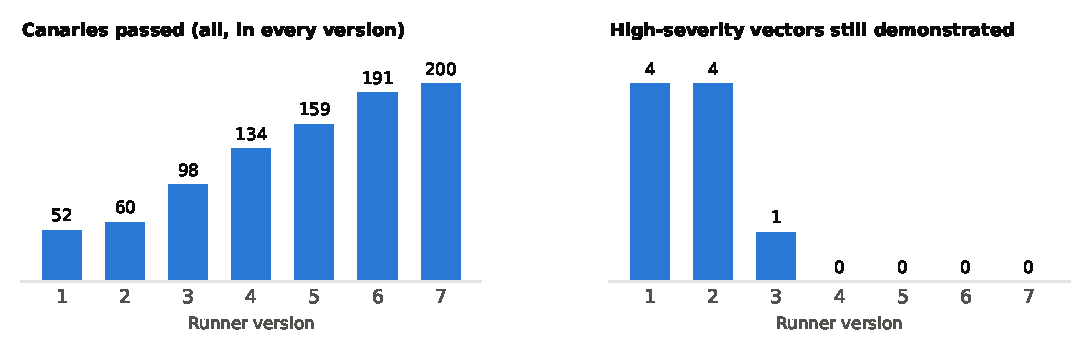
\includegraphics[width=\linewidth]{fig/runner_versions.pdf}
\caption{Canaries passed and high-severity vectors found, per runner version.}
\label{fig:versions}
\end{figure}


\textbf{Passing canaries proved little.} No attack escaped the container's namespaces or privileges in any round. Nine demonstrated high-severity vectors came through what the host shared with it: host-side steps that touched agent-written files, resource limits (a known class \cite{r13}) and the model server.

\textbf{Final version.} Controls on 481 tasks (reference patch 481/481, empty patch 0/481) showed no verdict, exit-code or test-summary difference from the previous version. After the runner was killed, the container was gone within 149 s with no further model request. The final runner completed a 24-job list at 251--254 runs per hour with 8 workers.

\textbf{What remains.} Containers share the host kernel; user namespaces are not remapped; the request parser runs in the trusted runner; a job can slow others through the shared model server within its caps. Our claim is conditional: against the stated adversary and with the eight hashes matching, no tested attack succeeded.

\section{Conform: eight checks against the scorer path}\label{sec:4}

\texttt{conform} reads the requests a local stack sent and, where logged, the prompts the server rendered. Reference values come from the public starter notebook \cite{r10}, our Kaggle-kernel traces, and the Kaggle model's chat template.

\begin{table}[!tb]
\centering
\caption{The eight checks.}\label{tab:2}
\footnotesize
\begin{tabular}{@{}
  >{\raggedright\arraybackslash}p{(\linewidth - 4\tabcolsep) * \real{0.1300}}
  >{\raggedright\arraybackslash}p{(\linewidth - 4\tabcolsep) * \real{0.5200}}
  >{\raggedright\arraybackslash}p{(\linewidth - 4\tabcolsep) * \real{0.3500}}@{}}
\toprule
\begin{minipage}[b]{\linewidth}\raggedright
Check
\end{minipage} & \begin{minipage}[b]{\linewidth}\raggedright
Compares
\end{minipage} & \begin{minipage}[b]{\linewidth}\raggedright
Mutation runs caught
\end{minipage} \\
\midrule
role & role of tool results & 53/53 \\
sampling & temperature, top-p, token and thinking budgets & 52/52 \\
tools & declared tool schemas & 20/20 \\
shape & message skeleton, system text, field encoding & 72/72 \\
template & rendered prompt against the Kaggle template & 13/21 by token count, 24/24 by token id \\
thoughts & history thoughts, under the key the server reads & 52/52 \\
newline & newline before the token closing a thought & 12/12 \\
compaction & when history is summarized (14,336 tokens \cite{r10}) & 19/19 \\
\bottomrule
\end{tabular}
\end{table}

\textbf{Role.} From each google-adk release's source (only 1.36.1 was executed): 1.34.0--1.39.1 and 2.0--2.4 send \texttt{tool\_responses} when the model string contains ``gemma4''; 2.5--2.11 when it matches \texttt{gemma-?4}; 2.12--2.14 exempt three OpenAI-compatible providers \cite{r5}. The harness packages require \texttt{\textgreater{}=1.34.0,\textless{}2.0}.

\textbf{Thoughts.} vLLM 0.19.1 reads an earlier assistant thought only from the field \texttt{reasoning}. google-adk 1.36.1 writes \texttt{reasoning\_content}, which that server drops silently \cite{r8}; the competition harness writes both. Removing \texttt{reasoning} in a probe lost 55 of 55 thoughts from the rendered prompt.

\textbf{Template.} The check re-renders each request outside vLLM with the Kaggle template and compares token counts with the server's, or token ids when the server logs them, because identical strings can tokenize differently \cite{r16}.

\textbf{Evidence.} In version 2's 24-task parity run, all 2,566 tool results had role \texttt{tool}, and re-rendering reproduced the server's token count on 396 of 396 requests (with \texttt{tool\_responses}: 0 of 358 multi-turn requests). With the final runner, the checker reproduced the token ids of 243 of 243 returned calls, and a renderer written separately by the verifier matched 50 of 50 scorer-path requests. Prompts rebuilt from early calls of our Kaggle-kernel traces match the recorded counts on 181 of 189 calls with role \texttt{tool} and thoughts kept, 1 of 189 with \texttt{tool\_responses} and 0 of 189 with thoughts dropped: our only Kaggle-side evidence, and count-level.

\textbf{Mutation suite.} 103 mutations (85 drifts, 18 benign controls) in four scripted scenarios against a mock server give 412 runs. The intended check caught 317 of 325 applicable drift runs; the 8 misses are same-length template changes seen through counts only. No check failed in 72 control runs (24 warned).

\section{Compare: a decision rule that respects repositories}\label{sec:5}

Tasks from one repository succeed and fail together. Clustered inference for model evaluations is prior art \cite{r19}; \texttt{compare} packages a small-cluster version with a frozen pass rule and its simulated behaviour.

Candidate and baseline run on the same tasks and repeats. A candidate passes only if (1) the mean gain is at least 2/58 (3.45 points, two leaderboard tasks); (2) one-sided p \ensuremath{\le} 0.025 under a null-imposed wild cluster bootstrap-t over repositories, with Rademacher weights and 9,999 draws \cite{r20,r21}; (3) at least three repositories gain and every leave-one-repository-out estimate is positive; (4) agent time stays within 1.2 times baseline and infrastructure errors do not rise; and (5) no repository loses two task-equivalents or more. Two panels were frozen before any outcome: a small one (72 tasks, 18 repositories) and a large one (200 tasks, 20 repositories).

\begin{table}[!tb]
\centering
\caption{Simulated pass rates (3,000 simulations per cell; 400 for the dropping row).}\label{tab:3}
\footnotesize
\begin{tabular}{@{}
  >{\raggedright\arraybackslash}p{(\linewidth - 4\tabcolsep) * \real{0.5800}}
  >{\raggedright\arraybackslash}p{(\linewidth - 4\tabcolsep) * \real{0.2100}}
  >{\raggedright\arraybackslash}p{(\linewidth - 4\tabcolsep) * \real{0.2100}}@{}}
\toprule
\begin{minipage}[b]{\linewidth}\raggedright
Simulated scenario
\end{minipage} & \begin{minipage}[b]{\linewidth}\raggedright
Small panel
\end{minipage} & \begin{minipage}[b]{\linewidth}\raggedright
Large panel
\end{minipage} \\
\midrule
No effect, exchangeable tasks & 0.23--1.90\% & 0.00--0.50\% \\
No mean effect, candidate breaks 20\% of repositories & 7.50\% & 8.43\% \\
No effect, worst tasks dropped after seeing outcomes & 31.75\% & 40.75\% \\
Even gain of 3/58 (power) & \ensuremath{\approx}60\% & \ensuremath{\approx}90\% \\
Gain confined to four repositories (power) & 15.9\% & 24.9\% \\
\bottomrule
\end{tabular}
\end{table}

The 2.5\% level holds for exchangeable effects, not for skewed ones, and not if tasks are dropped after unblinding. Independent re-implementations matched the rule code on 280 of 280 clean datasets (first version) and, with rule readings aligned, 193 of 194 (amended). Applied three times, to screen leaders from one separate 48-task set (25, 22, 25 of 96 runs solved; baselines 19, 21, 20); none passed. Gains: \ensuremath{-}0.35 points on the small panel (p = 0.60); on the 128 large-panel tasks outside it, \ensuremath{-}0.39 (p = 0.60), then +4.10 (p = 0.04 \textgreater{} 0.025, uncorrected). Condition (5): first application only.

\section{Case study: four prompt divergences on E4B}\label{sec:6}

Five arms share one model server, one withheld agent bundle, google-adk 1.36.1 and all sampling settings.

\begin{table}[!tb]
\centering
\caption{Arms; changes in percentage points.}\label{tab:4}
\footnotesize
\begin{tabular}{@{}
  >{\raggedright\arraybackslash}p{(\linewidth - 6\tabcolsep) * \real{0.0500}}
  >{\raggedright\arraybackslash}p{(\linewidth - 6\tabcolsep) * \real{0.4000}}
  >{\raggedright\arraybackslash}p{(\linewidth - 6\tabcolsep) * \real{0.1900}}
  >{\raggedright\arraybackslash}p{(\linewidth - 6\tabcolsep) * \real{0.3600}}@{}}
\toprule
\begin{minipage}[b]{\linewidth}\raggedright
Arm
\end{minipage} & \begin{minipage}[b]{\linewidth}\raggedright
Difference from the scorer path
\end{minipage} & \begin{minipage}[b]{\linewidth}\raggedright
Requests changed by the divergence
\end{minipage} & \begin{minipage}[b]{\linewidth}\raggedright
Change against F {[}95\% interval{]}; Holm p
\end{minipage} \\
\midrule
F & none: role \texttt{tool}, Kaggle template, compaction at 14,336 tokens, thoughts under both keys & --- & solve rate 23.8\% \\
R & model name contains ``gemma4'': tool results get role \texttt{tool\_responses} & 89\% & \ensuremath{-}0.3 {[}\ensuremath{-}2.8, +2.2{]}; p = 1 \\
C & compaction unset: prompts grow until rejected above 24,576 tokens (the run ends; edits are still graded) & 21\% & +0.2 {[}\ensuremath{-}2.0, +2.5{]}; p = 1 \\
H & history thoughts removed from every request, as when a client omits the key the server reads & 90\% & \ensuremath{-}2.1 {[}\ensuremath{-}4.4, +0.4{]}; p = 0.44 \\
T & the Hugging Face E4B template: a thought opener is forced after each tool result & 85\% & +0.8 {[}\ensuremath{-}1.4, +2.9{]}; p = 1 \\
\bottomrule
\end{tabular}
\end{table}

No newline arm was run: both templates render it identically on this server.

\textbf{Panel.} Removing tasks used by other panels, reserved repositories, slow tasks and duplicates from the 579 leaves 231 tasks in 15 repositories. They run 4 repeats in 5 arms (4,620 jobs); for each task and repeat the arms run back to back in counterbalanced order.

\textbf{Analysis, frozen before any outcome} (protocol sha256 \texttt{\seqsplit{070c9655d96372d054f430727259de7b25af2ca93c3ec4c9295dfdc37aeb8cf4}}). The estimand $d_X$ is the mean over tasks of arm X's solve rate minus arm F's. The primary test is an exact two-sided task-level sign-flip test, Holm-corrected over the four arms at 0.05; only then do we say that X raises or lowers E4B's solve rate \emph{on these tasks}. Intervals (unadjusted) invert that test. A repository-cluster bootstrap interval is secondary (lower simulated power). A frozen checker re-renders every returned request from the job's dump, matches the server's token count and confirms the job's arm; a failing job is re-run. Outcomes stayed blind until a pre-registered cut-off (2026-11-11 06:00 UTC) and were unblinded once.

\textbf{Power, simulated before data.} The family-wise false-claim rate is 1.2--4.2\%. At 231 tasks an even 5-point drop in one arm is detected with probability 82--100\% across the simulated settings; the drop or gain detected with 80\% power ranges from below 3 to about 5.2 points.

\textbf{Deviations recorded blind.} Independent validation of the final runner finished only after launch. From about an hour in, a second workload held about 9.6 GiB of GPU memory, so timings are under mixed load. The block stopped three times: after 967 jobs at the runner's open-file limit (cause unknown), after 378 more by an external termination signal on the shared machine, and after 3,074 more when the kernel's out-of-memory killer ended the model server (cause undiagnosed). Each resume ran only never-started jobs; the 24 interrupted jobs were re-run once.

\textbf{Results.} All jobs finished before the cut-off. Every arm has a valid row in 924 of 924 slots, and the checker passed all 4,620 analysed jobs. No pre-emption was recorded; 6.0\% of runs took over 240 s, above the pre-registered 5\% threshold. No difference from F was detected for any arm (Table~\ref{tab:4}, Figure~\ref{fig:parity}B; smallest Holm-adjusted p 0.44); the secondary repository-cluster intervals all include zero. The largest estimate is H's \ensuremath{-}2.1 points (unadjusted p 0.11; \ensuremath{-}1.3 with time-limit rows as missing). In exploratory measures, H runs averaged 137 s against 78 s and ended unsolved at the bundle's five-minute limit in 11.5\% of runs against 1.8\%; in C, 12.3\% of runs ended unsolved on a rejected over-long prompt. These are null results, not evidence of no effect: the simultaneous 98.75\% intervals allow a drop of 5.1 points (H) and a gain of 3.5 (T).

\begin{figure}[!tb]
\centering
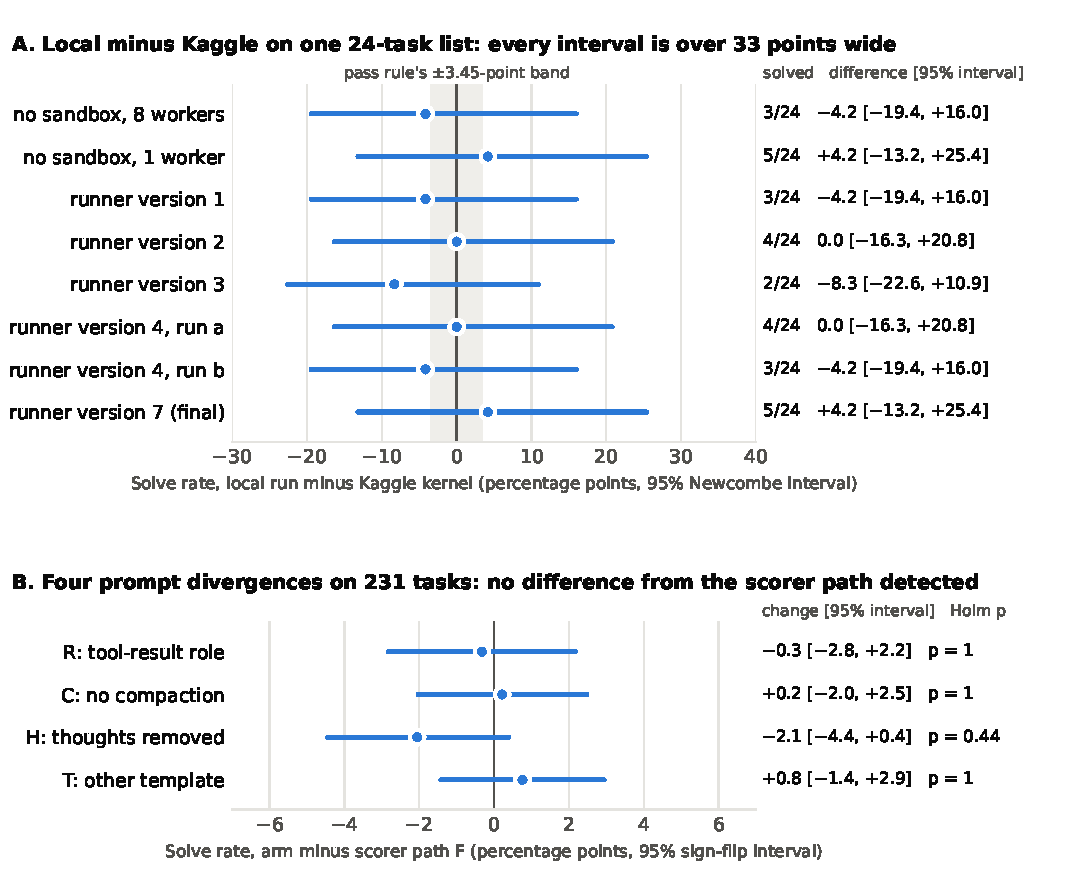
\includegraphics[width=\linewidth]{fig/parity_effects.pdf}
\caption{(A) Solve-rate difference, local minus Kaggle (pooled 8/48), for eight local runs of one 24-task list (95\% Newcombe intervals, runs treated as independent); shaded: the pass rule's \ensuremath{\pm}3.45 points. (B) Change in solve rate against F on 231 tasks: estimates, 95\% intervals and Holm-adjusted p.}\label{fig:parity}
\end{figure}

\section{Related work}\label{sec:7}

SandboxEval \cite{r14} and SandboxEscapeBench \cite{r15} test sandboxes and models' ability to escape them.

Several paper-track resources overlap this one (described from their public text only): LAB \cite{r22}, a Docker sandbox with 11 tests and a bundle gate with 16 detectors validated by fault injection; Szeto et al.'s cloud rig with 141 run folders \cite{r23}; gemma4-swe-kit \cite{r17}, a proxy reproducing the scorer's template, call parsing and compaction on other servers; a dataset card reporting count parity on 107 captured vLLM requests \cite{r18}; Silent Zeros \cite{r24}, a bundle checker tested on 22 broken bundles; and ThoughtKeep \cite{r25}, 1,470 Gemma 4 31B attempts on thought retention. We did not find in those texts, and offer here: a runner attacked by independent verifiers with its canary misses published, token-id comparison backed by a mutation suite, and a trap measurement on E4B with a per-job prompt check.

\section{Limitations}\label{sec:8}

\begin{itemize}
\tightlist
\item
  \textbf{Solve-level parity is not refuted, not established.} The evidence (Figure~\ref{fig:parity}A) is one 24-task list, one repeat per run; ten runs solved only six distinct tasks.
\item
  \textbf{Kaggle-side facts are partly inferred}: the hosted google-adk release, tool-schema equality, and the identity of the hosted template and weights with the public Kaggle model.
\item
  \textbf{Environment differences remain.} One RTX 5090 instead of four L4s; 2 CPUs and 10 GiB per job; a bare \texttt{pytest} command, used in 30 of 216 commands in our Kaggle traces, is absent locally.
\item
  \textbf{The case study} covers one model, one bundle, one google-adk release and one configuration per divergence. Arm T swaps a whole template; in arm H thoughts still reach compaction summaries.
\end{itemize}

\section{Availability}\label{sec:9}

\texttt{drydock-eval} 0.4.0 (Apache-2.0) has three modules: \texttt{conform} (checks, mock server, mutation suite), \texttt{contain} (a reference runner tree, its escape tests, a gate helper) and \texttt{compare} (pass rule, sign-flip tests, simulations). Its 435 CPU tests pass. The released runner has not been run in a container as released: the 200 of 200 result is for the deployed tree, of which the release is an identifier-substituted copy with two canaries rewritten. Code: \url{https://github.com/MinhThanghus/drydock-eval} (tag \texttt{v0.4.0}; branch \texttt{paper}: supplement, \S\ref{sec:6} outcome rows). The package also carries copies of the \S\ref{sec:6} protocol, analysis code and job-list generator, redacted where needed, each with its original's sha256; the agent bundle and request dumps are planned for 2026-12-03.
